%----------------------------------------------------------------------------------------
%	PACKAGES AND DOCUMENT CONFIGURATIONS
%----------------------------------------------------------------------------------------

\documentclass[10pt,a4paper]{article}
\usepackage[utf8]{inputenc}
\usepackage{graphicx} % Required for the inclusion of images
\graphicspath{{res/}}
\usepackage{natbib} % Required to change bibliography style to APA
\usepackage{amsmath} % Required for some math elements 
\usepackage{amsfonts}
\usepackage{amssymb}
\usepackage{listings}
\usepackage{float}

\usepackage[T1,T2A]{fontenc}

\setlength\parindent{0pt} % Removes all indentation from paragraphs

\renewcommand{\labelenumi}{\alph{enumi}.} % Make numbering in the enumerate environment by letter rather than number (e.g. section 6)

%----------------------------------------------------------------------------------------
%	DOCUMENT INFORMATION
%----------------------------------------------------------------------------------------

\title{Проект OWASP WebGoat} % Title

\author{Виктор \textsc{Борисов}} % Author name

\begin{document}

\maketitle % Insert the title, author and date

\newpage

\tableofcontents

\newpage

%----------------------------------------------------------------------------------------
%	SECTION 1
%----------------------------------------------------------------------------------------

\section{Цель работы}

Изучить описания 10 самых распространенных веб-уязвимостей согласно рейтингу OWASP.

\section{Ход работы}

\subsection{Изучение}

\subsubsection{Описания десяти самых распространенных веб-уязвимости согласно рейтингу OWASP}

\begin{itemize}

\item {\textbf{Injection} Атака на интепритатор машины-цели, позволяя выполнять произвольный код от ее имени. Чаще всего встрачаются в SQL, LDAP, Xpath, или NoSQL запросах, парсерах xml, аргументах программ и т.д.}
\item {\textbf{Broken Authentication and Session Management} Атака на уязвимости систем авторизации и управления сессиями с целью кражи и/или выполнения каких либо действий от чужого имени.}

\item {\textbf{Cross-Site Scripting} Атака на браузер путем подмены загружаемых скриптов. В результате злоумышлиниками может быть получена почти любая информация.}

\item {\textbf{Insecure Direct Object References} Суть атаки - изменение некого объекта, используемого в авторизированной сессии.

Изменение параметра позволит отправлять измененные запросы от имени авторизированного пользователя.}

\item {\textbf{Security Misconfiguration} Ошибки в конфигурации. Атакующий может получить доступ к файлам, акаунтам, системе и т.д.}

\item {\textbf{Sensitive Data Exposure} Кража ценной/личной информации. Атака сложна если используется шифрование. В таком случае данные крадутся косвенными методами: на стороне клиента, когда данные уже рашифрованы, man-in-the-middle атака и другими способами.}

\item {\textbf{Missing Function Level Access Control} Доступ неавторизированного пользователя к привелегированным функциям. }


\item {\textbf{Cross-Site Request Forgery} Атака путем выполнения запросов к некоторому защищенному ресурсу от его имени авторизованного пользователя. Недостаток - атакующий не может перехватить ответ от ресурса. В этом случае вводят так называемые CSRF-токены: каждый последующий пакет от клиента содержит токен, полученный в пердыдущем ответе сервера.}

\item {\textbf{Using Components with Known Vulnerabilities} Атака на уязвимый компонент системы, выявленный в результате сканирования.}

\item {\textbf{Unvalidated Redirects and Forwards} Скрытые ссылки в картинках, фреймах и т.д., ведущих на доверенный сайт. Позволяет произвести любой запрос.}

\end{itemize}

\subsection{Подготовка рабочей среды}
Необходимо заупстить и настроить  WebGoat, ZAP, Mantra.
WebGoat запущен на порту по умолчанию - 8080. ZAP настраивается на работу на 8081 порт. И такой же порт прописывается в настройках прокси в Mantra.

\begin{figure}[H]
\centering
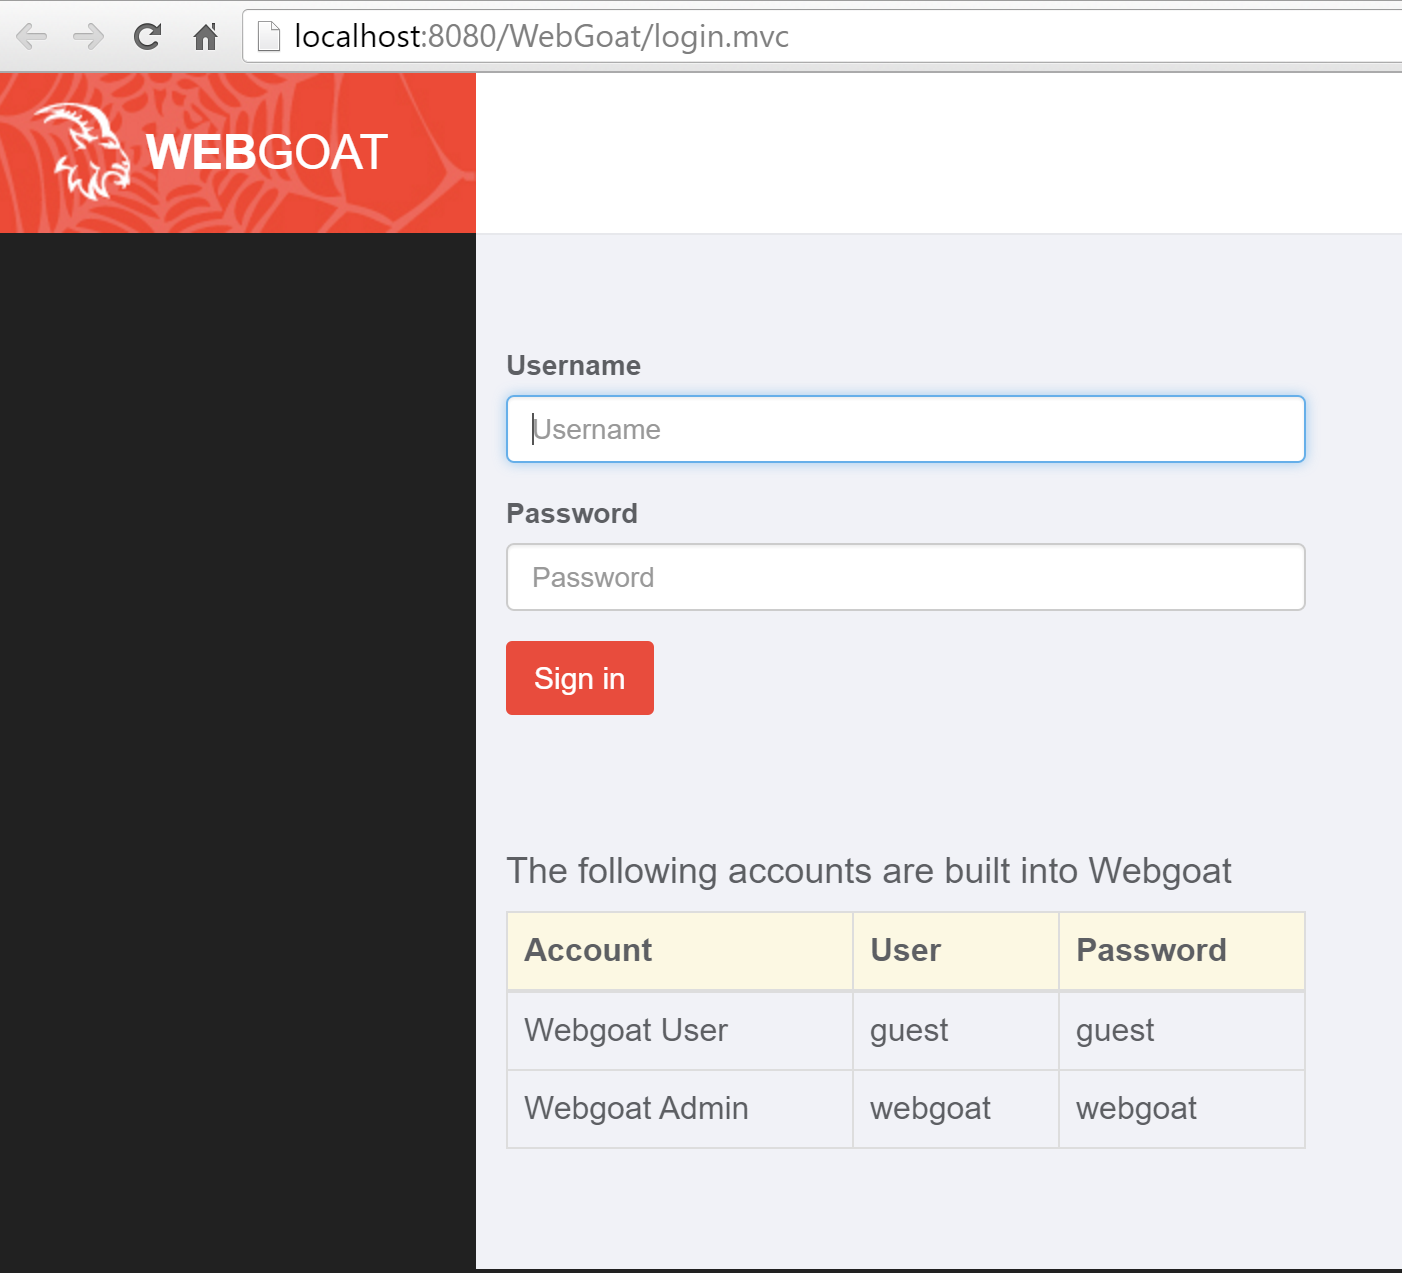
\includegraphics[width=\textwidth]{webgoat_homepage}
\caption{Запуск WebGoat}
\end{figure}

\begin{figure}[H]
\centering
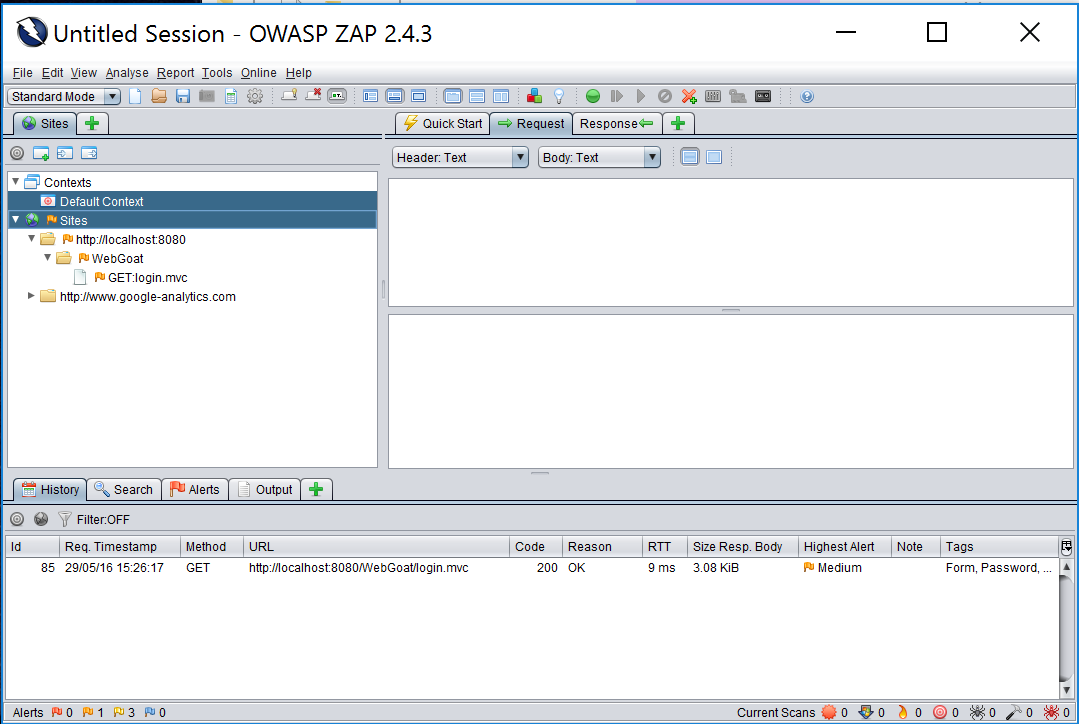
\includegraphics[width=\textwidth]{zap_started}
\caption{Запуск ZAP.}
\end{figure}

\begin{figure}[H]
\centering
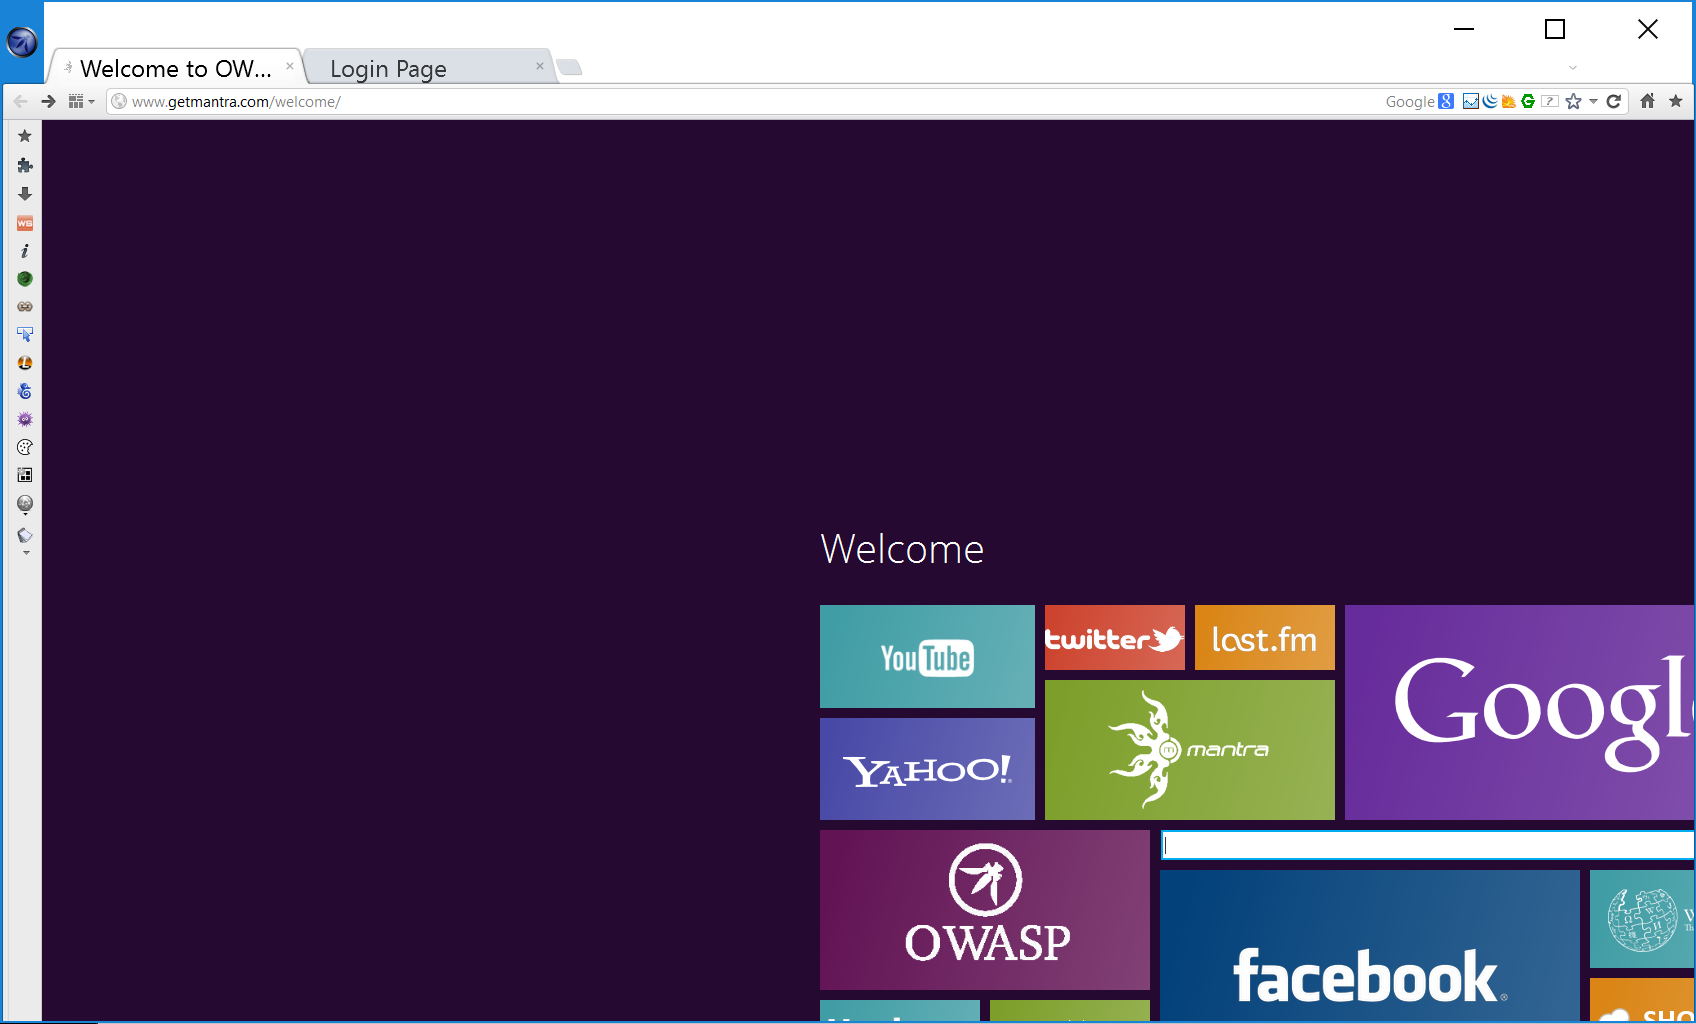
\includegraphics[width=\textwidth]{mantra_started}
\caption{Запуск Mantra.}
\end{figure}


\subsection{Практическое задание}

\subsubsection{Недостатки контроля доступа}

Bypass a Path Based Access Control Scheme

Получение доступа к файлу, находящемуся вне нашей директории. Для этого перехватим запрос и заменим имя файла на "../../../../WEB-INF/spring-security.xml". Доступ к файлу получен.

\begin{figure}[h]
\centering
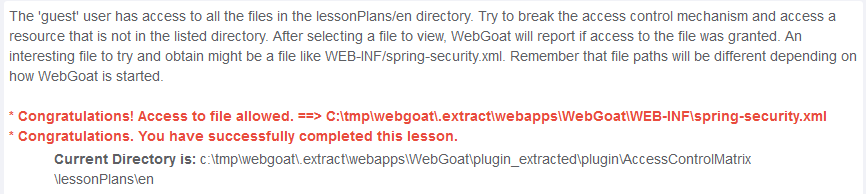
\includegraphics[width=\textwidth]{access_spring_security}
\caption{Доступ к файлу вне директории.}
\end{figure}

Bypass Bussines Layer Access

Заходим под аккаунтом, не имеющем права удаления, например, Tom (пароль tom), и, перехватывая запрос View Profile, подменим вызываемый метод на DeleteProfile. Профиль другого сотрудника удален. 

\begin{figure}[h]
\centering
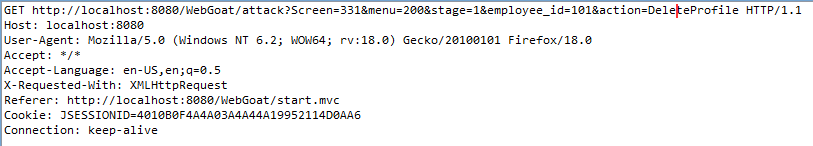
\includegraphics[width=\textwidth]{deleteProfile}
\caption{Удаление.}
\end{figure}

Bypass Data Layer Access

В данном задании необходимо подменить ID пользователя (аналогично предыдущему заданию), тем самым получив данные другого пользователя.

\subsubsection{Безопасность AJAX}

Client Side Filtering

Показывает недостатки фильтрации полученных данных на клиентской стороне. Так как можно получить информацию, непредназначенную для данного пользователя. 

Dom based cros-site scripring

Показывает необходимость экранирования входных данных. Например, выполнить произвольный html код.

\begin{figure}[h]
\centering
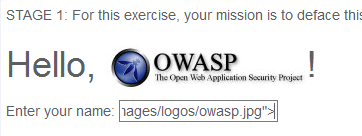
\includegraphics[width=\textwidth]{ajax_mg}
\caption{Результат подмены.}
\end{figure}

DOM injection

Показывает принцип работы DOM injection. Используя инъекцию можно изменить свойства элементов страницы. Например, изменить submit.disabled на false при помощи перехвата запроса и инъекции следующей строки:

\begin{verbatim}
document.forms[0].SUBMIT.disabled=false;
\end{verbatim}
Кнопка станет активной.

XML Injection

Показывает пример XML инъекции. В перехваченный запрос нужно вставить
\begin{verbatim}
<root>
<reward>WebGoat Mug 20 Pts</reward>
<reward>WebGoat t-shirt 50 Pts</reward>
<reward>WebGoat Secure Kettle 30 Pts</reward>
<reward>WebGoat Core Duo Laptop 2000 Pts</reward>
<reward>WebGoat Hawaii Cruise 3000 Pts</reward>
</root>
\end{verbatim}

JSON Injection

Аналогично предыдущему заданию, но теперь JSON инъекция
\begin{verbatim}
{
"From": "Boston",
"To": "Seattle",
"flights": [
{"stops": "0", "transit" : "N/A", "price": "$20"},
{"stops": "2", "transit" : "Newark,Chicago", "price": "$300"}
]
}
\end{verbatim}




Третья часть урока показывает, что необходимо делать валидацию данных не только на клиенте, но и на сервере, чтобы исключить подмену ajax-запросов. Изменив скрипт обработки запроса мы исключили возможность выдачи лишних данных клиенту.




Седьмая часть - не стоит делать проверку на клиентской стороне. Необходимо найти клиентскую функцию для отправки и вызвать ее.
\begin{verbatim}
submitData(555, 1000000)
\end{verbatim}

Insecure client storage

Показывает, что не стоит использовать вводимые поля помеченные атрибутом disabled или readonly, так, например, можно изменить стоимость товара при оплате.


Dangerous use of eval

Опасность функции eval

\begin{verbatim}
`)%3Balert(document.cookie
\end{verbatim}

\subsubsection{Недостатки аутентификации}

Password strength

Показывает зависимость сложности подбора пароля от его длины и набора символов.

Forgot password

Показывает, что механизм восстановления пароля не должен быть простым, иначе нет смысла в сложном пароле.

Multi level login 1

При перехвате пакета выставляем hiddentan=1 и получаем список TAN.

Multi level login 2

Авторизуемся под пользователем Joe и используем его TAN, перехватыем пакет и изменяет пользователя на Jane.

\subsubsection{Переполнение буфера}
Перехватываем пакет, добавляем в значение аргумента roomno >4096 символов.

\subsubsection{Качество кода}
В коде страницы можно найти логин и пароль администратора.

\subsubsection{Многопоточность}
Thread safety problem

При одновременной работе нескольких пользователей возможно перемешивание получаемых данных. Открываем два окна и вводим имена пользователей. В некоторых случаях можно получить чужие данные.

Shopping cart concurrency flew

Открываем два окна, в одном делаем большую покупку, в другом - маленькую. Продолжаем маленькую покупку и обновляем большую. При подтверждении платим за маленькую, а получаем большую покупку.

\subsubsection{Межсайтовое выполнение сценариев}
С помощью XSS и HTML можно заменять элементы страницы на фиктивные, при этом пользователь не заметит изменений.

\subsubsection{Неправильная обработка ошибок}
В перехваченном пакете достаточно удалить поле пароля и авторизация пройдет успешно.

\subsubsection{Недостатки приводящие к осуществлению инъекций (SQL и прочее)}
\begin{itemize}
\item Command injection
Перехватываем запрос, добавляем к имени файла строку:
\begin{verbatim}
%22%3B%20netstat%20-a
\end{verbatim}
\item Numeric SQL injection
Перехватываем запрос. Модифицируем:
\begin{verbatim}
station=101or%201%3D1&SUBMIT=Go!
\end{verbatim}
\item Log spoofing
Перехватываем запрос, меняем имя на следующее:
\begin{verbatim}
somename
Admin succefully entered!
\end{verbatim}
В результате, в логе создается видимость того, что админ авторизовался.
\item SQL Injection
Перехватываем сообщение. В качестве пароля вводим:
\begin{verbatim}
123123%27%20OR%20%271%27%3D%271
\end{verbatim}
При попытке получить данные на втором шаге получаем сообщение:
\begin{verbatim}
THIS LESSON ONLY WORKS WITH THE DEVELOPER VERSION OF WEBGOAT
\end{verbatim}
\item String sql injection
Аналогично. Вместо имени вводим 12345' OR 'a' = 'a. Получаем все возможные значения.
\item Modify Data with SQL INJECTION
Вместо имени вводим:
\begin{verbatim}
UPDATE salaries SET salary=5 WHERE userid='jsmith
\end{verbatim}
\item Database backdoors
По такой же схеме можно добавлять и триггеры:
\begin{verbatim}
101; CREATE TRIGGER bckDoor BEFORE INSERT ON employee FOR EACH ROW BEGIN UPDATE employee SET email='john@hackme.com' WHERE userid = NEW.userid
\end{verbatim}
\end{itemize}


\subsubsection{Отказ в обслуживании}
ZipBomb

Создается файл zip, содержащий большое количество одинаковых символов. Такой тип файлов хорошо поддается сжатию, поэтому при распаковке займет очень много дискового пространства. 

DoS from Multiple logins

Используем инъекцию: вместо пароля вводим
\begin{verbatim}
12345' or `1' or `1
\end{verbatim}

Возвращается
\begin{verbatim}
101 jsnow passwd1
102 jdoe passwd2
103 jplane passwd3
104 jeff jeff
105 dave dave
\end{verbatim}
Авторизуемся этими данными. Получаем отказ в обслуживании из-за большого количества сессий.

\subsubsection{Небезопасное сетевое взаимодействие}
При передаче пароля вне защищенного соединения его можно легко перехватить, для избежания этого необходимо использовать https + TLS. 

\subsubsection{Небезопасная конфигурация}

Показывает необходимость сокрытия расположения панели администирования, чтобы предотвраить нежелательный доступ к ней.

\subsubsection{Небезопасное хранилище}

Показываются различные алгоритмы кодирования текста.

\subsubsection{Исполнение злонамеренного кода}
ВОзможность загрузки собственного скрипта и выполнение его.
\begin{verbatim}
<html>
<%
java.io.File fil = new java.io.File("c:\tmp\webgoat\.extract\webapps\WebGoat\mfe_target\guest.txt");
file.createNewFile();
%>
</html>
\end{verbatim}

\subsubsection{Подделка параметров}
Bypas HTML Field Restrictions

При перехвате пакета изменить значение полей и добавить disabledinput.

Exploit Hidden Fields 

Аналогично.

Exploit unchecked email

В поле собщения вводим тело скрипта
\begin{verbatim}
<script>alert("hi")</script>
\end{verbatim}
Для отправки скрипта на другой адрес меняем в перехваченном пакете значение аргумента "to":
\begin{verbatim}
gId=GMail+id&gPass=password&subject=Comment+for+WebGoat&
to=friend%40owasp.org&msg=%3Cscript%3Ealert%28%22hi%22
%29%3C.script%3E&SUBMIT=Send%21
\end{verbatim}

Bypass Client Side JavaScript Validation 

Аналогично.

\subsubsection{Недостатки управление сессией}

Hijack a Session 

Задание показывает необходимость использования сложных механизмов генерации пользовательских идентификаторов, чтобы нельзя былл с легкостью перехватить чужую сессию.

Session fixation 

Отправка электронного письма, содержащего в себе ссылку с добавленным SID (Session ID). После того как жертва осуществит вход по данной ссылке нам будет доступна сессия с переданным нами ID.

\subsubsection{Безопасность веб-сервисов}

\newpage

\section{Выводы}
В ходе работы было с помощью средства WebGoat были изучены и отработаны наиболее распространненые уязвимости веб-приложений, а так же способы их устранения.


\end{document}

